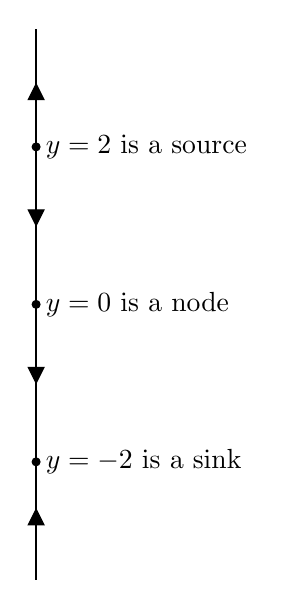
\begin{tikzpicture}[scale=1]
\draw[thick] (0,-3.5) -- (0,3.5);
\filldraw (0,0) node[right] {$y = 0$ is a node} circle (0.05);
\filldraw (0,2) node[right] {$y = 2$ is a source} circle (0.05);
\filldraw (0,-2) node[right] {$y = -2$ is a sink} circle (0.05);
\filldraw (0,1) -- (-0.1, 1.2) -- (0.1, 1.2) -- cycle;
 \filldraw (0,-1) -- (-0.1, -0.8) -- (0.1, -0.8) -- cycle;
\filldraw (0,-2.6) -- (-0.1, -2.8) -- (0.1, -2.8) -- cycle;
 \filldraw (0,2.8) -- (-0.1, 2.6) -- (0.1, 2.6) -- cycle;
\end{tikzpicture}